\section{Data source}\label{data-source}
The biggest initial task for this thesis was the acquisition of data.
Selecting a data source was a crucial step, as good data for analysis and evaluation is the backbone of this thesis.
This section will list all requirements in detail and evaluate why I chose to use Github as a data source.
Furthermore some functionalities of Github will be explained and a brief overview of the data provided by Github's \ac{api} will be given.


\subsection{Requirements}\label{requirements}
The data source had to satisfy as many requirements, which were specified in Chapter~\ref{attack-models}, as possible.

To accomplish a meaningful analysis of commit conduct one needs a sufficient amount of commits.
For instance it is necessary to have a few commits per weekday over a timespan of a month for a simple sleep rhythm analysis.
If there are only 20 commits for a user over the past month there is probably not enough data for a representative analysis.
To gather as many commits as possible we have to get access to as many repositories to which the targeted user contributed to as possible.
Thereby the data source has to provide a way to dynamically explore repositories around a single user.

For analysis of companioned persons as described in Section~\ref{industrial-spy} it is crucial to find users, which are likely to know each other.
Optimally the data source provides a functionality for users to actively mark other users as their friends or colleagues.

To attack a company, as described in Section~\ref{industrial-spy}, or to spy on company members, as described in Section~\ref{employer-monitoring}, the best case scenario would be to have full access to all repositories owned by the company.
The data source thereby needs to provide some kind of representation for a company.
Ideally there should also be a list of all company members for evaluation purposes of data mining findings.


\begin{itemlist}{A summary of the requirements to the data source:}
    \item Real world data
    \item Large amount of repositories
    \item Access to all commits of each repository
    \item Access complete metadata for each commit
    \item Email address to user association
    \item Methods to discover repositories a user contributed to
    \item Methods to discover possibly companioned contributor
    \item A representation of a company
    \item Access to members of a company
\end{itemlist}


\subsection{Github}\label{github}
I decided to use Github as a data source, for it is not only convenient to find \acp{url} for cloning repositories, but also provides solutions for most of the other requirements.
It hosts one of the biggest collections of open source projects~\cite{techreport:how-github-conquered} with 64 million repositories, 24 million users and 1,5 million organizations~\cite{article:github-statistics}.
Github also provides a well documented \ac{api} for querying its metadata and there are libraries for most major languages, which provide an abstraction layer for this \ac{api}.
This \ac{api} is publicly available and can be used by anyone registered on Github.

For instance Gitlab, one of Github's competitors, has much less data to offer.
Gitlab does not provide detailed usage statistics, but they state that they only host about 100000 organizations, which is remarkably less than Github~\cite{article:gitlab-help}.
As Gitlab is an open-source project and anyone can host their own private Gitlab instance, there is an unknown number of privately hosted Git repositories, which are completely unaccessible for unauthorized users.

On the other hand one of the downsides of using Github is, that we do not have access to all metadata.
For example the full list of members for organizations is often unaccessible, as users actively need to opt-in to be publicly displayed as a member of the team.
The internal team structures of organizations are not visible, as one needs to be a member of the organization to access those.
Another problem are dangling email addresses, which are not related to any account any more.
All commits made with this email address cannot be used any more for any analysis which requires a user to commit relationship.
Even though some ground truth is missing, I decided to use this approach as it still was the most promising way to gather as much data and real world noise as possible, compared to other open source hosting services.

\begin{figure}[H]
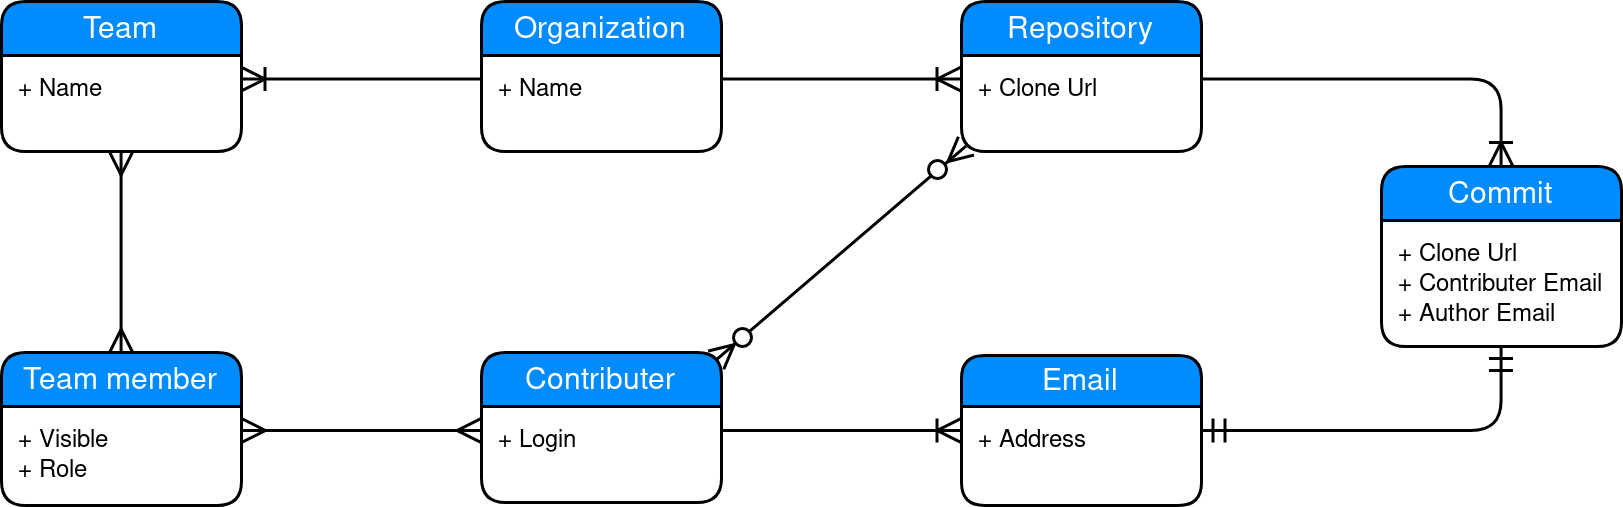
\includegraphics[scale=0.27]{./graphs/github-data-structure}
\centering
\caption{Simplified Github relationships in Crow's foot notation.}\label{fig:github-relationship}
\end{figure}

\subsection{Github's Features}\label{github-features}
In the following I will explain some of the features provided by Github, which cover the requirements listed in Section~\ref{requirements}.
Github offers some features, which are convenient to for example find repositories a specific user contributed to or to find contributors which likely personally know each other.

\begin{description}
    \item[Stars] \hfill \\
        A very crucial feature is \emph{starring}. Every user has the possibility to star a repository to show appreciation or interest in this specific project.
        Hence popular repositories usually have a comparative big amount of stars. For instance the Github Linux kernel mirror has a star count of over 58000~\footnote{`Linux kernel source tree' Github.com, https://github.com/torvalds/linux (accessed, 24.04.2018)}.
        Even though Github allows to query all repositories, which are owned or forked by a user, their \ac{api} does not provide a method to get all repositories a user ever contributed to.
        However Github provides an endpoint to query all starred repositories of an user.
        In case a user stars a repository he contributed to, whilst not owning it, it is now possible to get this repository with this feature.
        Of course it is still not a reliable way to get all repositories a user ever contributed to, but it is a viable approach to get at least a few of them.

    \item[Follower] \hfill \\
        Another important feature is \emph{following}.
        Every user can follow any other user to get informed, if they do specific things, like creating new repositories or starring repositories, or to simply show interest in or respect for their work.
        By getting all followed or following users, one might catch some friends of the user.
        It is also possible that a user follows the owner of a repository he contributed to.
        By using this feature it is thereby possible to get some additional contributed repositories as well some friends of the user.

    \item[Organizations] \hfill \\
        The third feature are \emph{organizations}.
        An organization is used to host projects under an account, which is not necessarily led by a single natural person, but rather supports roles with different permissions and team structures.
        Github allows to query all repositories of an organization via their \ac{api}.
        This enables us to link an organization to its owned repositories and as a result to perform analyses for users on a specific organization repository subset.

        Generally organizations provide us with some important ground truth, even though the information might not be complete.
        Despite not knowing all members of an organization, we still get some useful information to estimate the tendency of precision of our knowledge extraction algorithms.
\end{description}
